
\begin{figure}[h!]
    \centering
    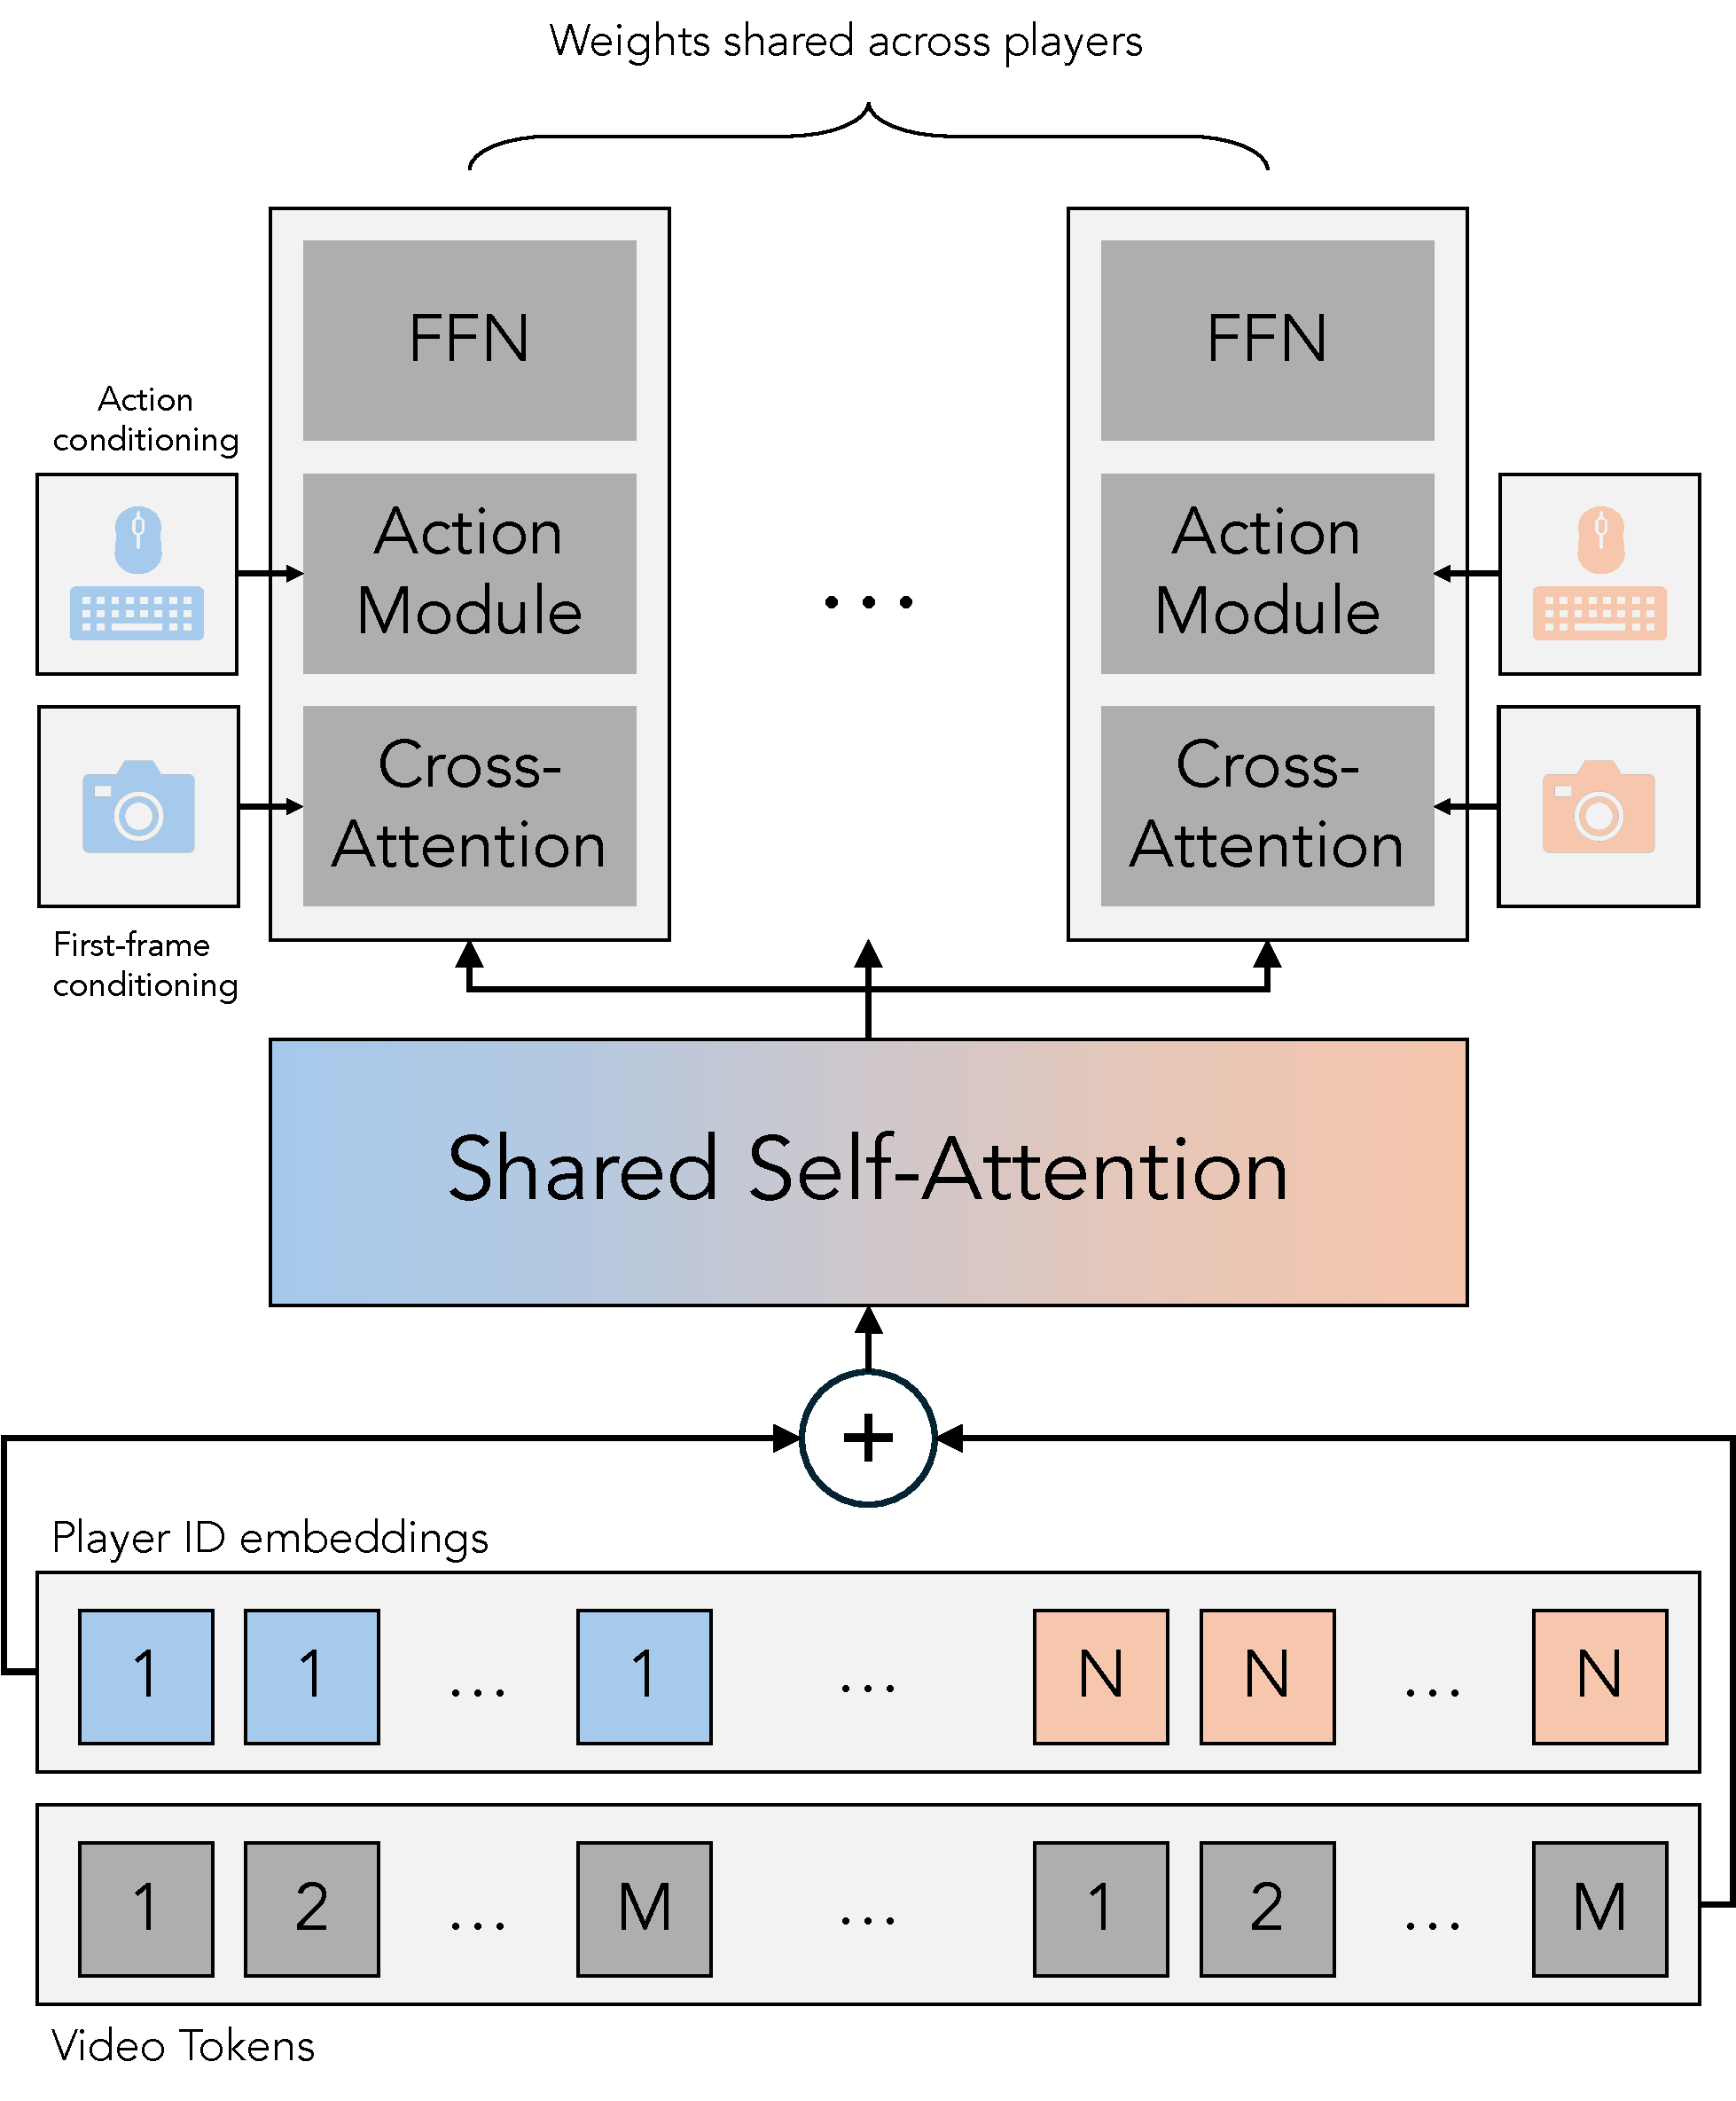
\includegraphics[width=0.5\linewidth]{figs/assets/arch.pdf}
    \caption{Our modified DiT block achieves multiplayer modeling through visual interleaving along the sequence dimension. We denote the number of players with $N$ and the number of tokens per video with $M$. Multiplayer information is exchanged through a shared self-attention block. The other modules are unchanged from \matrixgame and applied independently per player.}
    \label{fig:arch}
\end{figure}


\section{\solaris Model Design}
\label{sec:solaris_model}

\subsection{Preliminaries}
We consider a world model that can predict the future observations of multiple agents given their past observations and actions. While a traditional autoregressive diffusion model operates on a latent frame $\mathbf{x}_{\text{SP}} \in \mathbb{R}^{H \times W \times C}$, we generalize this to the multi-agent setting by augmenting the state space to include an extra player dimension $\texttt{P}$, performing diffusion on a joint tensor of shape $\texttt{(P, H, W, C)}$. Let $\mathbf{x}^t = \{x_1^t, \dots, x_P^t\}$ denote the joint state and $\mathbf{a}^{t} = \{a_1^t, \dots, a_P^t\}$ the joint actions of all $P$ agents at time $t$. Let $\mathbf{x} \coloneqq \mathbf{x}^{1:T}$ and $\mathbf{a} \coloneqq \mathbf{a}^{1:T}$ denote the combined tensor of consecutive latent observation and action tensors across a sequence of length $T$. Thus $\mathbf{x}$ has shape \texttt{(B, P, T, H, W, C)} and $\mathbf{a}$ has shape \texttt{(B, P, T, D)}. We model the probability distribution $p_\theta(\mathbf{x}) = \prod_{t=1}^{T} p_\theta(\mathbf{x}^t \mid \mathbf{x}^{<t}, \mathbf{a}^{<t})$ using a diffusion model. We restrict $P=2$ in this work, though our framework is flexible enough to be generalizable to any number of players.


We train our model with conditional Flow Matching~\cite{liu2022flow,lipman2022flow}. Concretely, we optimize the loss
\[
\mathcal{L}_\theta = \mathbb{E}_{\mathbf{x}, \mathbf{a},\sigma, \epsilon} \left[ \left\| v_\theta(\mathbf{x}_{\boldsymbol{\sigma}}, \boldsymbol{\sigma}, \mathbf{a}) - (\epsilon - \mathbf{x}) \right\|_2^2 \right],
\]
using the standard forward process $\mathbf{x}_{\boldsymbol{\sigma}} = (1 - \boldsymbol{\sigma})\mathbf{x} + \boldsymbol{\sigma}\epsilon$ where $\epsilon\sim \mathcal{N}(\mathbf{0}, \mathbf{I})$. The noise schedule differs depending on the model variant. For our \emph{bidirectional} model, we use a shared noise level across all players and frames: $\sigma \sim \mathcal{U}(0, 1)$, with $\boldsymbol{\sigma} = \sigma \cdot \mathbf{1}_{ P \times T}$, so that all elements are noised and denoised jointly. For our \emph{causal} model, we adopt Diffusion Forcing~\cite{chen2024diffusionforcingnexttokenprediction} to enable autoregressive generation, sampling independent noise levels per player and per frame: $\boldsymbol{\sigma} \in [0, 1]^{P \times T}$, where each entry $\sigma_{p,t} \sim \mathcal{U}(0, 1)$ is independent. 




\subsection{Network Architecture}
\label{subsec:model_architecture}

Our architecture is built on \matrixgame~\cite{he2025matrixgame20opensourcerealtime}, a single-player controllable video Diffusion Transformer~\cite{peebles2023scalablediffusionmodelstransformers} (DiT) model that was trained on multiple video games, including Minecraft. A visualization of our multiplayer DiT block can be found in~\cref{fig:arch}. To adapt \matrixgame to be capable of multiplayer modeling, we introduce several changes which we discuss below. 

\textbf{Expanded action space.} We extend the action space of \matrixgame to use the full range of Minecraft actions encoded as the MineRL~\cite{guss2019minerllargescaledatasetminecraft} action space by increasing the input dimension of the \matrixgame keyboard action module and reinitializing its weights. We run the action module independently per-player, folding the player dimension into the batch. In psuedocode, this is achieved through \texttt{rearrange("B P T D -> (B P) T D")}.  

\textbf{Multiplayer attention.} Information across different players is exchanged through Multiplayer Self-Attention layers in our DiT blocks. We apply 3D RoPE~\cite{su2024roformer} to each player's tokens \textit{independently} and inject player information by adding learned player ID embeddings to each player's tokens at the start of each Multiplayer Self-Attention layer. The cross-attention block, which provides first-frame conditioning, remains unchanged from \matrixgame and is applied independently per-player. 
